\documentclass[11pt,a4paper]{article}
\usepackage[T1]{fontenc}
\usepackage{lmodern}
\usepackage[latin1]{inputenc}
\usepackage{a4wide}
\usepackage[dvips]{graphicx}
\usepackage{float}

\usepackage[
pdfauthor={},
pdftitle={},
pdfcreator={pdftex},
]{hyperref}

\usepackage{sectsty}
\allsectionsfont{\sffamily}

\usepackage{fancyheadings} 
\pagestyle{fancy} 
\lhead{\textsf{\textbf{ACE} \\ \small{a collaborative editor}}}
\chead{}
\rhead{
\parbox[c]{3cm}{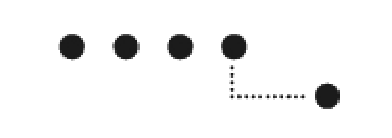
\includegraphics[height=0.875cm,width=3cm]{../../images/logo_BFH.eps}}
\parbox[c]{2.2cm}
{\tiny{\textsf{Berner Fachhochschule \\
Hochschule f�r \\
Technik und Informatik}}}}
\lfoot{}
\cfoot{\textsf{\thepage}}
\rfoot{}
\setlength{\headrulewidth}{0.6pt}
\setlength{\footrulewidth}{0.6pt}
\setlength{\topmargin}{-50pt}
\addtolength{\headheight}{50pt}

\usepackage{colortbl}

\newcommand{\headercol}[2]{\multicolumn{1}{|>{\bfseries\columncolor[gray]{0.82}}p{#1}|}{\textsf{#2}}}
\newcommand{\ace}[0]{\emph{ACE }}



\begin{document}
\setlength{\parindent}{0pt}

\begin{titlepage}
\thispagestyle{empty}
  
\includegraphics[height=1.5in]{../images/pix.eps}

  \begin{center}

    {\fontsize{40}{45} \textbf{\textsf{ACE}}} \\
    \textsf{a collaborative editor} \\
        
    \vspace{36pt}
        
    {\huge{\textbf{\textsf{}}}} \\

    \vspace{36pt}

	\textsf{Berne University of Applied Sciences} \\
    \textsf{School of Engineering and Information Technology} \\
    
  \end{center}

  \vfill
  
  \begin{tabular}{ll}
   \hline

   \\

   \multicolumn{1}{>{\bfseries}p{1.5in}}{\textsf{Date:}} &
   \multicolumn{1}{>{}p{4.3in}}{\textsf{08.11.2005}}          \\
   
   \\
   
   \multicolumn{1}{>{\bfseries}p{1.5in}}{\textsf{Version:}}     &   
   \multicolumn{1}{>{}p{4.3in}}{\textsf{0.1}}                 \\

   \\
   
   \multicolumn{1}{>{\bfseries}p{1.5in}}{\textsf{Projectteam:}}                 &
   \multicolumn{1}{>{}p{4.3in}}{\textsf{Mark Bigler (biglm2@hta-bi.bfh.ch)}}  \\
   \multicolumn{1}{>{\bfseries}p{1.5in}}{}                                      &
   \multicolumn{1}{>{}p{4.3in}}{\textsf{Simon Raess (rasss@hta-bi.bfh.ch)}}    \\
   \multicolumn{1}{>{\bfseries}p{1.5in}}{}                                      &
   \multicolumn{1}{>{}p{4.3in}}{\textsf{Lukas Zbinden (zbinl@hta-bi.bfh.ch)}} \\   
   
   \\
   
   \multicolumn{1}{>{\bfseries}p{1.5in}}{\textsf{Receivers:}}                       &
   \multicolumn{1}{>{}p{4.3in}}{\textsf{Jean-Paul Dubois (doj@hta-bi.bfh.ch)}}       \\
   \multicolumn{1}{>{\bfseries}p{1.5in}}{}                                          &
   \multicolumn{1}{>{}p{4.3in}}{\textsf{Claude Fuhrer (frc@hta-bi.bfh.ch)}}       \\

   \\
   
   \multicolumn{1}{>{\bfseries}p{1.5in}}{\textsf{Location:}}               &   
   \multicolumn{1}{>{}p{4.3in}}{\textsf{Subversion Repository}} \\

   \\  
   
   \hline
  \end{tabular}

\end{titlepage}

\newpage

\tableofcontents
\newpage

\listoftables
\listoffigures
\newpage



\section{Introduction}
Testing distributed systems can be complicated. The order of events in the system are generally non deterministic. In the literature about collaborative editing, sessions are depicted as in figure \ref{fig:session}.

\begin{figure}[H]
 \centering
 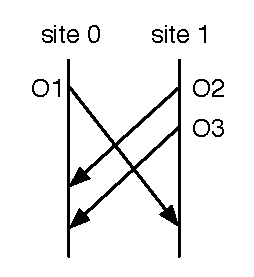
\includegraphics[width=3.7cm,height=4.1cm]{../../images/testframework_puzzle.eps}
 \caption{Collaborative editing session}
 \label{fig:session}
\end{figure}

In order to implement a collaborative application, one should be able to specify such scenarios (testcases) with expected results (final states). This is the reason why we decided to implement a testframework.

Effectively the test framework will allow to test the operational transformation algorithm implementation. This is the core part of a collaborative editing application. Other parts of the system will have to be tested otherwise and are intentionally left out.


\subsection{Requirements}
The testframework has the following basic requirements:
\begin{itemize}
 \item specify scenarios as depicted in figure \ref{fig:session}
 \item specify initial and final states
 \item verify that final states are equal at the end at all sites
\end{itemize}
Further the following requirements are given:
\begin{itemize}
 \item independent of algorithm implementation (testframework uses only 
       abstract and application independent classes and interfaces)
 \item applicable to any algorithm implementation
\end{itemize}
If not all the aspects of a given algorithm implementation can be tested by the testframework, specific tests have to be written.



\section{Architecture}
The central classes of the test framework are:

\begin{itemize}
 \item ScenarioLoader
 \item ScenarioBuilder
 \item Node
 \item NodeVisitor
 \item Scenario
\end{itemize}

The \texttt{ScenarioLoader} is responsible to load a scenario from a given input stream. The default implementation (\texttt{DefaultScenarioLoader}) loads the scenario from an XML file. The \texttt{ScenarioLoader} has a single method \texttt{loadScenario}. This method accepts a \texttt{ScenarioBuilder} and as input an input stream.

The \texttt{ScenarioBuilder} is the interface needed to build a scenario. The \texttt{ScenarioLoader} uses this abstract interface to inform the builder about the structure of the scenario. The default implementation \texttt{DefaultScenarioBuilder} creates a \texttt{Scenario} object, which is an object model for a scenario. The default scenario builder represents the scenario as a graph. The nodes of the graph have specific semantic meaning. There are nodes for generation of operations, reception of messages and messages for the start/end of a site's lifecycle.

The \texttt{Scenario} object built by the \texttt{DefaultScenarioBuilder} contains the nodes topologically sorted. That is, ancestors are visited before their children. 

\texttt{Scenario} has a method \texttt{accept} that takes a \texttt{NodeVisitor} as a parameter. The \texttt{NodeVisitor} has methods for all the existing node types. It gets called back for each node in the scenario. 

The \texttt{ExecuteVisitor} executes a given scenario. That is, it replays the scenario on a given algorithm implementation. The \texttt{AlgorithmTestFactory} is used to create the algorithm implementation object for each site. It has also methods for creating documents and timestamps.


\subsection{Scenario Graph}
To understand the inner workings of the \texttt{ch.iserver.ace.test} package, one must know the structure of a scenario. A scenario consists of vertical lines that represent the lifecycle of a site. On these vertical lines, there are certain events. These events can be seen as nodes in the graph. From generation events there are edges both to the next local event and edges to all remote sites (send events). The reception of a message (represented by a reception node) are another type of node.

The scenario graph has a special property. It is a directed acyclic graph. This special property is a necessary condition to check on a generated scenario object model. It is used to process the graph in topological order.

\begin{figure}[H]
 \centering
 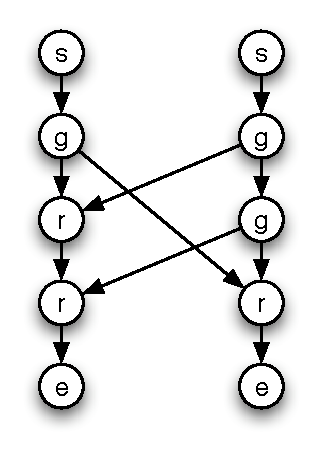
\includegraphics[width=4.9cm,height=7.2cm]{../../images/testframework.eps}
 \caption{Scenario Graph}
 \label{fig:graph}
\end{figure}

So the scenario from figure \ref{fig:session} is transformed into the scenario graph in figure \ref{fig:graph}. There are four different types of nodes: start (s), generation (g), reception (r) and end nodes (e). The start nodes represent the start of the lifecycle of a site, the generation nodes the generation of an operation, the reception nodes the reception of a remote request and the end nodes the end of a site's lifecycle. 


\subsection{Node Structure}
The nodes of the scenario graph are represented by the \texttt{Node} interface. There are four implementations of this interface: \texttt{StartNode}, \texttt{GenerationNode}, \texttt{ReceptionNode} and \texttt{EndNode}. The nodes store the successors but not the predecessor. This information is not needed for traversing the nodes in topological order. A distinction is made between local and remote successors in order to facilitate testing of some properties on the graph.


\subsection{Properties to Test}
There are several properties that have to be checked on the generated scenario object in order to be sure that the scenario is correct. That is, given a correctly working algorithm implementation, the replayed scenario results in converging document states at all sites.

\paragraph{GenerationNode}
A \texttt{GenerationNode} must have the following properties:
\begin{itemize}
 \item exactly one predecessor node (local)
 \item exactly on local successor node
 \item exactly $n - 1$ remote successor nodes
 \item that is there must be exaclty $n$ successor nodes
\end{itemize}

\paragraph{ReceptionNode}
A \texttt{ReceptionNode} must have the following properties:
\begin{itemize}
 \item exactly two predecessor nodes, one local, one remote
 \item exactly on successor nodes
\end{itemize}

\paragraph{StartNode}
A \texttt{StartNode} has the following properties:
\begin{itemize}
 \item no predecessor
 \item exactly one successor
\end{itemize}
Note that these properties are not explicitely checked by the implementation.

\paragraph{EndNode}
An \texttt{EndNode} has the following properties:
\begin{itemize}
 \item exactly one predecessor
 \item no successor
\end{itemize}
Note that these properties are not explicitely checked by the implementation.

\paragraph{Other Checks}
Beside the basic checks on the nodes, the following checks have to be done:
\begin{itemize}
 \item no operation is generated and received at the same site
 \item no operation is received more than once by same site
 \item no operation is generated twice
 \item generated graph is a directed acyclic graph
\end{itemize}



\section{How To}
This section contains information on both how to create a scenario definition in the standard format (XML file) expected by \texttt{DefaultScenarioLoader} and how to use scenario defininitions for tests of concrete algorithm implementations.

\subsection{XML Scenario Definition}
The default implementation of \texttt{ScenarioLoader} loads scenario definitions from an xml file. The XML file conforms to the XSD schema found at \texttt{/src/resources/test/scenario.xsd} in the subversion repository. Following is an example of a scenario document:

\begin{verbatim}
<?xml version="1.0"?>
<scenario initial="ABC" final="AcB">
    <operation id="1" type="ch.iserver.ace.text.Insert">
        <property name="position" value="1"/>
        <property name="text" value="c"/>
    </operation>
    <operation id="2" type="ch.iserver.ace.text.Delete">
        <property name="position" value="2"/>
    </operation>
    <site id="0">
        <generate ref="1"/>
        <receive ref="2"/>
    </site>
    <site id="1">
        <generate ref="2"/>
        <receive ref="1"/>
    </site>
</scenario>
\end{verbatim}

The root element \texttt{scenario} defines the initial and final state at all sites. It has two type of child elements, \texttt{operation} and \texttt{site}. All operations have to be declared. The operation element has an \texttt{id} attribute uniquely identifying the operation and a type attribute that specifies what Java object should be instantiated. The \texttt{property} child elements allow to set properties on the created operation objects. The \texttt{name} attribute specifies the property name and the \texttt{value} attribute specifies the value of the property.

The \texttt{site} element has an \texttt{id} attribute that is used only for informational purpose. A \texttt{site} element can contain \texttt{generate} and \texttt{receive} elements, both of which have a \texttt{ref} attribute identifying an operation by identifier. The sequence of \texttt{generate} and \texttt{receive} elements inside a \texttt{site} element represent the sequence of events at one site. 

Based on this information in the XML file the scenario graph can be created. The XML schema file itself contains documentation about the structure of XML scenario files.


\subsection{Test Algorithm Implementation}
In the package \texttt{ch.iserver.ace.test} there is a JUnit abstract test case subclass called \texttt{AlgorithmTestCase}. This class has a single protected method \texttt{execute} that executes a given scenario. It uses the default scenario loader and default scenario builder. 

To create a test case for a specific algorithm implementation, you should make the following steps:

\begin{enumerate}
 \item create subclass of \texttt{AlgorithmTestCase}
 \item add implementation for methods of \texttt{AlgorithmTestFactory} interface.
       This includes methods for creating the algorithm, initial timestamps
       and document models.
 \item add test methods calling execute with the corresponding scenario
       as input
\end{enumerate} 

The execute methods throws \texttt{VerificationException} if there was an error verifying the final state at all sites. That is, the document state diverged. A \texttt{ScenarioException} is thrown if there is an error loading/building the scenario.


\end{document}
